\documentclass{article}
\usepackage[legalpaper, margin=1cm]{geometry}
\usepackage{amsmath,amssymb,amsthm}		% If AMS-LaTeX is used, this comes first
\usepackage{color}

\usepackage{enumitem}
\usepackage{graphicx}
\setlist[itemize]{noitemsep, topsep=0pt}
\newcommand{\topic}[1]{\textbf{\underline{#1}}}
\newcommand{\R}{\mathbb R}
\newcommand{\Z}{\mathbb Z}
\newcommand{\N}{\mathbb N}
\newcommand{\p}{\partial }
\newcommand{\grad}{\nabla}
\newcommand{\Ex}{\underline{Example:} }
\newcommand{\ex}{\underline{Ex:} }
\newcommand{\dx}{\text{ dx }}
\newcommand{\dt}{\text{ dt }}
\newcommand{\dfn}{\underline{Definition:} }
\newcommand{\thm}{\underline{Theorem:} }
\newcommand{\Note}{\underline{Note:} }
\newcommand{\note}{\underline{Note:} }
\newcommand{\FS}{\sin \Big( \frac{n \pi x}{L} \Big)}
\newcommand{\FC}{\cos \Big( \frac{n \pi x}{L} \Big)}
\graphicspath{ {./images/} }
\title{Partial Differential Equations - Class Notes}
\date{\today}
\author{Steven Blythe}

\begin{document}
\maketitle
\newpage
\section{Chapter 1}
\subsection*{Sidenotes}
\subsection*{January 19, 2022}
\topic{What is a PDE?}\\
A PDE is an equation which contains partial derivatives of an unknown function and we want to find that unknown function.\\
\Ex $F(t, x, y, z, u, \frac{\partial u}{\partial t}, \frac{\partial u}{\partial x}, \frac{\partial u}{\partial y}, \frac{\partial u}{\partial z}, \frac{\partial^2 u}{\partial t^2}, \frac{\partial^2 u}{\partial x \partial y}, \ldots) = 0$.\\
Note, the first partial derivatives are considered \underline{$1^{st}$ ordered partials}\\
whereas the second ordered partials are considered \underline{$2^{nd}$ ordered partials}.\\
The variables that are not $u$ are considered independent variables and $u$ is considered a dependent variable.\\
What PDEs do we study?\\
Generally, we restrict our attention to equations that model some phenomenom from physics, engineering, economics, geology, \ldots\ etc. We can use physical intuition to help guide the math.\\
\topic{Classification of PDEs}
\begin{enumerate}
  \item Order of PDE: Highest derivative.\\
  \Ex $\frac{\partial^3 u}{\partial x^3} - \sin(y) u^7 = 3$ is a third order PDE.\\
  \Ex $(\frac{\partial y}{\partial t})^5 - \frac{\partial^2y}{\partial x \partial t} = e^x$ is a second order PDE.
  \item Number of independent variables.\\
  \Ex $\frac{du}{dt} = \frac{\partial^2 u}{\partial x^2}$ has two independent variables: $t, x$.\\
  This is the $1-D$ heat equation.\\
  \Ex $\frac{\partial u}{\partial t} = \frac{\partial^2 u}{\partial x^2} + \frac{\partial^2 u}{\partial y^2} + \frac{\partial^2 u}{\partial z^2} = \Delta u$ has 4 independent variables.\\
  This is the $3-D$ heat equation. $\Delta u$ is Laplacian of $u$.\\
  \underline{Notation}\\
  $
  \Delta u =
  \grad^2 u =
  \grad \cdot \grad u =
  (\frac{\partial}{\partial x}, \frac{\partial}{\partial y}, \frac{\partial}{\partial z}) \cdot (\frac{\partial u}{\partial x}, \frac{\partial u}{\partial y}, \frac{\partial u}{\partial z}) =
  \frac{\partial^2 u}{\partial x^2} + \frac{\partial^2 u}{\partial y^2} + \frac{\partial^2 u}{\partial z^2}
  $\\
  $\Delta u = 0$ is considered Laplace's equation.
  \item Linear vs non-linear\\
  A linear PDE is any equation of the form $L[u(x)] = f(x)$ where $f(x)$ is a known function is a linear partial differential operator.
\end{enumerate}
\dfn A differential operator is any rule that takes a function as its input and returns an expression that involves the derivatives of that function.\\
\Ex
\begin{align}
  u(x, t) & \qquad v(x, t)\\
  O[u] & = \frac{\partial^2 u}{\partial x^2} + \sin x + \pi - 7e^{tu}\\
  O[u + 3v] & = \frac{\partial^2}{\partial x^2}(u + 3v) + \sin x + \pi - 7e^{tu + 3tv}\\
  & = \frac{\partial^2 u}{\partial x^2} + 3 \frac{\partial^2 v}{\partial x^2}+ \sin x + \pi - 7e^{tu + 3tv}
\end{align}
\dfn A linear operator, L, is an operator that has the property:
\begin{align}
  L[au + bv] & = aL[u] + bL[v]
\end{align}
Where $a$ and $b$ are constants.\\
\thm If $u$ and $v$ are vectors and $L$ is linear, then $L$ can be represented by a matrix.\\
\thm If $L$ is linear ordinary operator, it must take the form:
\begin{align}
  L[u] = f_0(x)u + f_1(x)u^\prime + f_2(x)u^{\prime\prime} + \ldots + f_n(x)u^{(n)}
\end{align}
Where the $f_i$'s are known functions.\\
\dfn A linear ODE is any ODE of the form where $f(x)$ is known is the following:
\begin{align}
  L[u] = f(x)
\end{align}
If $f(x) = 0$, then the equation is homogeneous. Otherwise, the equation is non-homogeneous.\\
\ex $(u^\prime)^2 = 0 \Rightarrow u^\prime = 0 \rightarrow$ linear, homogeneous.\\
\thm If $L$ is a linear partial differential operator, it must take the form ($x$ is a vector with $n$ unknowns)
\begin{align}
  L[u(x)] = f_0(x)u + \sum^n_{i = 1} f_i(x) \frac{\partial u}{\partial x_i} +
  \sum^n_{i = 1} \sum^n_{j = 1} f_{ij}(x) \frac{\p^2 u}{\p x_i \p x_j} + \ldots
\end{align}
\dfn A linear PDE is any PDE of the form
\begin{align}
  L[u(x)] = f(x)
\end{align}
If $f(x) = 0$, the equation is homogeneous, else it is non-homogeneous.\\
\ex $u_t = 4u_x$ - Linear, homogeneous.
\newpage
\subsection*{January 21, 2022}
\Ex
\begin{align}
  u_{tt} & = u_{xx} + u{yy}\quad \text{Linear, homogeneous}\\
  \cos{(xt)} & = u + u_t + u_{xyz}\quad \text{Linear, non-homogeneous}\\
  u_tu_{xt} & = 0\quad \text{non-linear}\\
  u_{xt} + e^x \cos t\ u_t & = 0\quad \text{linear, homogeneous}\\
  u_t + u_{xx} + ue^u & = 0\quad \text{non-linear}
\end{align}
\note You can add linear combinations of solutions to linear homogeneous equations and still get a solution.
\Ex $u_x = u_t$.\\
Some solutions to this are:
\begin{enumerate}
  \item $u_1(x, t) = 3$
  \item $u_2(x, t) = x + t$
  \item $u_3(x, t) = e^{x+t} \cos(x + t)$
  \item $\qquad \vdots$\\
  $Au_1 + Bu_2 + Cu_3$ is also a solution.
\end{enumerate}
\topic{How do we solve an ODE?}
\begin{enumerate}
  \item Use some technique to find an explicit solution.
  \item Use power series and determine the coefficients
  \begin{align}
    y(x) & = \sum^\infty_{n = 0} a_nx^n
  \end{align}
  \item Laplace Transforms
\end{enumerate}
\topic{How do we solve PDEs?}
\begin{enumerate}
  \item Try to locate an explicit solution
  \item We don't use power series, instead, we use a trigonometric series $\Rightarrow$ Fourier Series.
  \begin{align}
    y(x) & = \sum^\infty_{n = 0} a_n \sin(nx) + b_n \cos(nx)
  \end{align}
  \item Laplace Transforms are good if the domain is $[0, \infty)$.\\
  Fourier Transforms are good if the domain is $(-\infty, \infty)$.
  \item Reduce the PDE to a system of ODEs.
\end{enumerate}
\topic{Initial Condiction}
\begin{enumerate}
  \item For ODEs, to solve a $1^{st}$ order equation, you need $y(0)$.\\
  $2^{nd}$ order $\rightarrow y(0), y^\prime(0)$\\
  $3^{rd}$ order $\rightarrow y(0), y^\prime(0), y^{\prime\prime}(0)$\\
  $\vdots$\\
  $n^{th}$ order $\rightarrow y(0), y^\prime(0), y^{\prime\prime}(0), \ldots, y^{(n - 1)}(0)$
  \item For PDEs, it's more complicated $\Rightarrow$ it depends on the PDE.\\
  \Ex $u(x, t), x \in [a, b], t \in [0, \infty)$\\
  If $u_t = u_{xx}$
  \item Boundary conditions:
  \begin{align}
    u(a, t) & = g_1(t)\\
    u(b, t) & = g_2(t)
  \end{align}
  If $u_{tt} = u_{xx}$, we must specify:
  \begin{enumerate}
    \item Initial Conditions
    \begin{align}
      u(x, 0) & = f_1(x)\\
      u_t(x, 0) & = f_2(x)
    \end{align}
    \item Boundary Conditions
    \begin{align}
      u(a, t) & = g_1(t)\\
      u(b, t) & = g_2(t)
    \end{align}
  \end{enumerate}
\end{enumerate}
\topic{1-D Heat Equation}\\
Assume cross sections are uniform
Imagine a cross section:
\begin{center}
  O o==========o L
\end{center}
Assume cross sections are uniform and the lateral sides are well insulated $\Rightarrow$ heat only flows in the x-direction.\\
We need the following:
\begin{itemize}
  \item $u(x, t)$ : Temperature of rod at position $x$ and time $t$.
  \item $u(x, 0)$ : Initial temperature
  \item $u(0, t)$ and $u(L, t)$ : Boundary Conditions
\end{itemize}
\dfn
\begin{itemize}
  \item $g(x, t)$ : heat flux (energy / area time)
  \item $Q(x, t)$ : heat energy density (energy / volume)
  \item $A$ : Cross sectional area
  \item $C_P$ : Heat capacity or specific heat
  \item $\rho$ : Density
  \item $K$ : Thermal conductivity
\end{itemize}
We want to find an equation for the temperature evolution. We will use conservation of energy : Look at a little $\Delta x$ section of the rod starting at $x_0$.
\begin{center}
  $\Delta x$\\
  o=====$|$o$|$=====o\\
  $x_0\  x_0\Delta x$
\end{center}
Conservation of energy : heat in - heat out = heat accumulated\\
Heat in $ = 'qA\Delta t' = A \int_{t_0}^{t_0 + \Delta t} q(x_0, t) \text{ dt}$\\
Heat out $ = A\int_{t_0}^{t_0 + \Delta t} q(x_0 + \Delta x, t) \text{ dt}$\\
Heat Accumulated $ = QA\Delta x |_{t_0 + \Delta t} - QA\Delta x|_{t_0}$
\begin{align}
  & = A\int^{x_0 + \Delta x}_{x_0} Q(x, t_0 + \Delta t) \text{ dx} - A\int^{x_0 + \Delta x}_{x_0} Q(x, t_0) \text{ dx}
\end{align}
\newpage
\subsection*{January 24, 2022}
\topic{Heat Equation}\\
\topic{Conservation of energy}\\
Heat in - heat out = heat accumulated
\begin{align}
  A \int^{t_0 \rightarrow \Delta t}_{t_0} g(x_0, t) \dt -
  A \int^{t_0 \rightarrow \Delta t}_{t_0} q(x_0 + \Delta x, t) \dt =
  A \int^{t_0 \rightarrow \Delta t}_{t_0} Q(x, t_0 + \Delta t) \dx -
  A \int^{t_0 \rightarrow \Delta t}_{t_0} Q(x, t_0) \dx
\end{align}
Let us simplify and divide by $A$. Then, let us combine the integrals:
\begin{align}
  \int^{t_0 \rightarrow \Delta t}_{t_0} [q(x_0, t) - q(x_0 + \Delta x, t)] \dt =
  \int^{t_0 \rightarrow \Delta t}_{t_0} [Q(x, t_0 + \Delta t) - Q(x, t_0)] \dx
\end{align}
Divide by $\Delta x \Delta t$ and take limit as $\Delta x, \Delta t \rightarrow 0$
\begin{align}
  \lim_{\Delta t, \Delta x \rightarrow 0} \frac{1}{\Delta x \Delta t}
  \int^{t_0 \rightarrow \Delta t}_{t_0} [q(x_0, t) - q(x_0 + \Delta x, t)] \dt & =
  \lim_{\Delta t, \Delta x \rightarrow 0} \frac{1}{\Delta x \Delta t}
  \int^{t_0 \rightarrow \Delta t}_{t_0} [Q(x, t_0 + \Delta t) - Q(x, t_0)] \dx\\
  \lim_{\Delta t} \frac{1}{\Delta t} \int^{t_0 \rightarrow \Delta t}_{t_0} [\lim_{\Delta x \rightarrow 0} \frac{q(x_0, t) - q(x_0 + \Delta x, t)}{\Delta x}] \dt & =
  \lim_{\Delta x \rightarrow 0} \frac{1}{\Delta x}
  \int^{t_0 \rightarrow \Delta t}_{t_0} \lim_{\Delta t \rightarrow 0} \frac
  {Q(x, t_0 + \Delta t) - Q(x, t_0)}{\Delta t} \dx
\end{align}
On the left side, we see the order is a bit difference. We want the delta to come first, such as in the difference quotient. The eft is now $-q_x(x_0, t)$ and the right is $Q_t(x, t_0)$.
\begin{align}
  \lim_{\Delta t \rightarrow} \frac{1}{\Delta t} \int^{t_0 + \Delta t}_{t_0} - q_x(x_0 t) \dt & =
  \lim_{\Delta x \rightarrow 0} \frac{1}{\Delta x} \int^{x_0 + \Delta x}_{x_0} Q_t(x, t_0) \dx\\
  \lim_{\Delta t \rightarrow 0} -q_x(x_0, t_0 + \Delta t) & = \lim_{\Delta x \rightarrow 0} Q_t(x_0 + \Delta x, t_0)
\end{align}
At step 28, we used the fundamental theorem of calculus and derived both sides.
\begin{align}
  -q_x(x_0, t_0) & = Q_t(x_0, t_0)
\end{align}
Since $x_0$ and $t_0$ are arbitrary, $-q_x(x, t) = Q_t(x, t)$\\
$q$ and $Q$ are related to $u$:
\begin{align}
  Q = \rho c_p u \qquad & \qquad q = -Ku_x\\
  -q_x = Q_t & \Rightarrow Ku_{xx} = \rho c_p u_t\\
  & \Rightarrow u_t = \frac{k}{\rho c_p} u_{xx}\\
  & \Rightarrow u_t = \alpha^2 u_{xx}\\
  \alpha & = \sqrt{\frac{K}{\rho c_p}}
\end{align}
$\alpha$ is thermal diffusivity\\
$u_t = \alpha^2 u_{xx} \leftarrow$ 1-D heat equation (diffusivity equation)\\
We have a steady-state: $(t \rightarrow \infty)$, $u_t = 0 \Rightarrow u_{xx} = 0 \Rightarrow $ straight line\\
1-D: $-q_x = Q_t \Rightarrow -\grad \cdot \vec q = Q_t, \qquad \vec q$ is a vector.
\begin{align}
  q = -K \grad u & \Rightarrow - \grad \cdot (-K \grad u) = \rho c_p u_t\\
  & \Rightarrow K \Delta u = \rho c_p u_t\\
  & \Rightarrow u_t = \alpha^2 \Delta u
\end{align}
What about a steady-state? $u_t = 0$
\begin{align}
  \Delta u & = 0
\end{align}
Here, we have Laplace's equation.\\
\note It is not dependent on time.\\
\topic{The Wave Equation}
$u(x, t)$ is the height of the rope. We use Newton's $2^{nd}$ law on small segments of rope.
\begin{itemize}
  \item $\rho = $ density of rope.
  \item $\text{dm} = \rho \dx$
\end{itemize}
% Image here
\begin{align}
  F & = ma\\
  T \sin(\theta(x + \Delta x)) - T \sin(\theta(x)) & = \int^{x + \Delta x}_x u_{tt} \text{ dm}\\
  T[ \sin(\theta (x + \Delta x)) - \sin(\theta (x))] & = \rho \int^{x + \Delta x}_{x} u_{tt} \dx
\end{align}
Let us assume $\theta$ is small, $\sin \theta \approx \tan \theta$
\begin{align}
  T[\tan(\theta(x + \Delta x)) - \tan(\theta(x))] & = \rho \int^{x + \Delta x}_x u_{tt} \dx
\end{align}
Also, $\tan(\theta(x)) = u_x(x, t)$.
\begin{align}
  T[u_x(x + \Delta x, t) - u_x(x, t)] & =
  \rho \int^{x + \Delta x}_x u_{tt} \dx
\end{align}
Now, let us divide both sides by $\Delta x$ and take the limit as $\Delta x \rightarrow 0$
\begin{align}
  \lim_{\Delta x \rightarrow 0} T\Big[\frac{u_x(x + \Delta x, t) - u_x(x, t)}{\Delta x}\Big] & =
  \rho \lim_{\Delta x \rightarrow 0} \frac{\int^{x + \Delta x}_x u_{tt} \dx}{\Delta x}
\end{align}
On the left side, we have $u_xx$ and the right side we have $u_{tt}(x + \Delta x, t)$.
\begin{align}
  Tu_{xx}(x, t) & = \rho u_{tt}(x, t)\\
  u_{tt} = \frac{T}{\rho} u_{xx} & = c^2 u_{xx}\\
  c & = \sqrt{\frac{T}{\rho}} = \text{ wave speed }
\end{align}
On the left, we have the $1-D$ wave equation which is used for light, sound, rope, etc.\\
In 2-D, it corresponds to a vibrating membrane (drum)
\begin{align}
  u_{tt} & = c^2\Delta u
\end{align}
\underline{Remark}:
\begin{align}
  u_t = u_{xx} \quad & \text{Heat Equation}\\
  u_{xx} + u_{yy} = 0 \quad & \text{ Laplace Equation}\\
  u_{tt} = u_{xx} \quad & \text{ wave}
\end{align}
Here, we can replace:\\
$u_t$ with $t$\\
$u_x$ with $x$\\
$u_{xx}$ with $x^2$
\begin{enumerate}
  \item $t = x^2$ parabola
  \item $x^2 + y^2 = 0$ ellipse
  \item $t^2 = x^2$ hyperbolas
\end{enumerate}
So, the equations behave like the following:
\begin{enumerate}
  \item The Heat Equation is called parabolic
  \item The Laplace Equation is called elliptic
  \item The Wave Equation is called hyperbolic
\end{enumerate}
\newpage
\subsection*{January 26, 2022}
\topic{Approximating Functions with other Functions}
\begin{enumerate}
  \item Prove Series
\end{enumerate}

  \begin{align}
    f(x) = \sum^M_{n = 0} a_n x^n \quad \text{Finite Power Series}
  \end{align}

  This is not the best way to approximate a function.

  We choose the $a_n$'s so that the power series is ``close'' to $f(x)$ which means we want to minimize the error.

  We increase $M$ to get a better approximation.

  The problem begins when you change $M$, the values of $a_n$'s change as well. Therefore, recalculating is a lot of work.

  If we let $M \to \infty$ and if $f \in C^\infty$, so then $a_n = \frac{f^{(n)}(0)}{n!}$ and we get the Taylor series.

  \note $C^\infty$: C means Continuous and the $\infty$ indicates the number of derivatives that are continuous.

  Problem: This is only good inside the radius of convergence.
  %
  \bigbreak
  %
  A Fourier Series is a trigonometric polynomial
  %
  \begin{align}
    \sum_{n = 0}^M a_n \FS + b_n \FC \longleftarrow \text{period = } 2L
  \end{align}

  We use Fourier Series for a function on a bounded interval and we will use $x \in [-L, L]$

  \topic{Advantages of Fourier Series}
  \begin{enumerate}
    \item If $M$ increases, we only need to calculate the new $a_n$'s and $b_n$'s. This property is due to the fact that the basis functions are orthogonal.

    \item If $M = \infty$ and $f$ is continuous, then the Fourier Series $= f(x) \forall x \in (-L, L)$. Our interval must be open for the case that $f(-L) \neq f(L)$.
  \end{enumerate}

  Basis Functions : $\FS, \FC$
  \begin{center}
    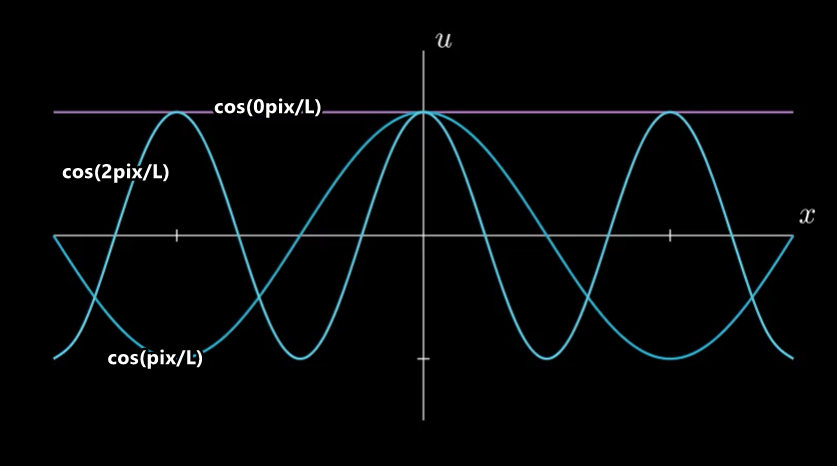
\includegraphics[height=5cm]{Fourier Basis Functions}
  \end{center}

  What happens if you use a Fourier Series on a discontinuous function?
  \begin{align}
    f(x) & =
    \begin{cases}
      1 & x \in (-4, 6)\\
      0 & x \in [-10, -4] \bigcup [6, 10]
    \end{cases}
  \end{align}

  \begin{center}
    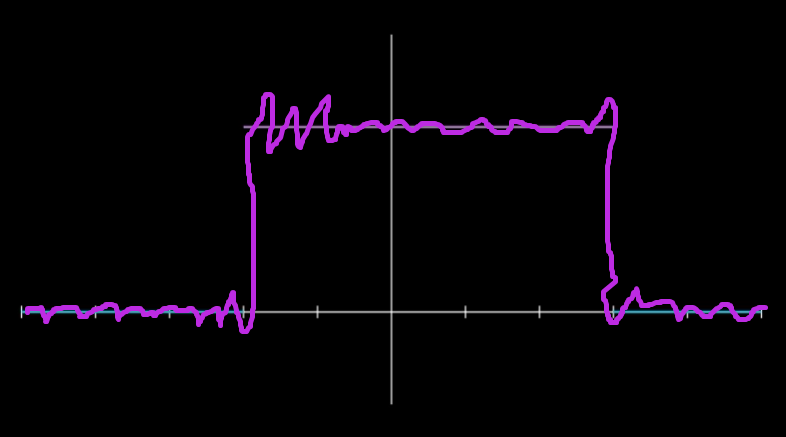
\includegraphics[height=5cm]{Fourier Finite Fourier Series}
  \end{center}

  The Oscillations around the discontinuities are called Gibbs phenomenon. As $M$ increases, the oscillation's amplitude does not change. However, the oscillations do get progressively closer to the discontinuities.

  \begin{center}
    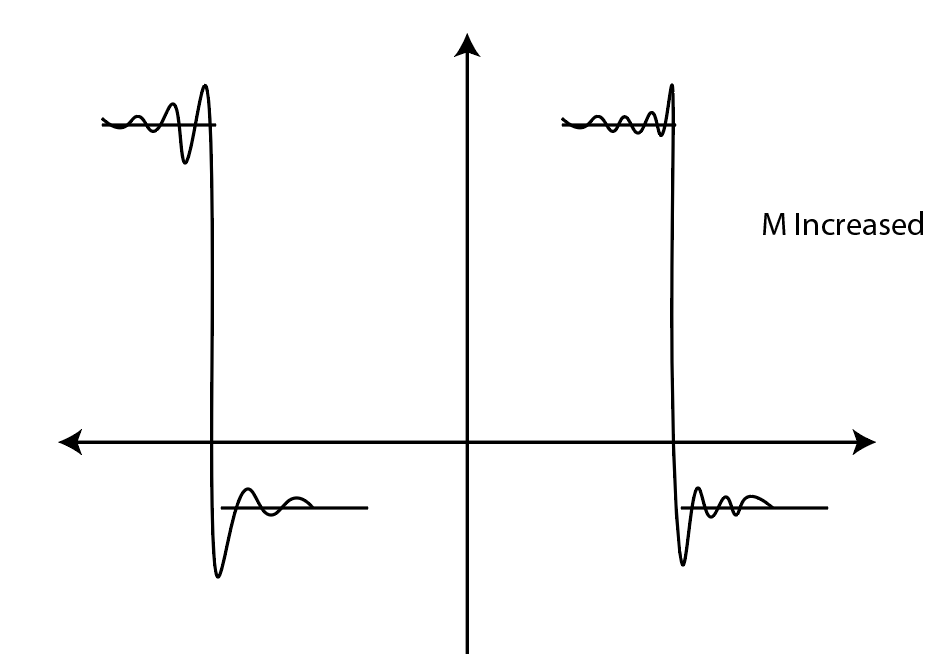
\includegraphics[height=5cm]{Fourier M}
  \end{center}

  If $M = \infty$, then we have:
  \begin{align}
    \text{Fourier Series } =
    \begin{cases}
      f(x) & = \text{ if $x$ is a point of continuity }\\
      \lim_{c \to 0^+} \frac{f(x + c) + f(x - c)}{2} & \text{ if x is a point of discontinuity}
    \end{cases}
  \end{align}

  \begin{center}
    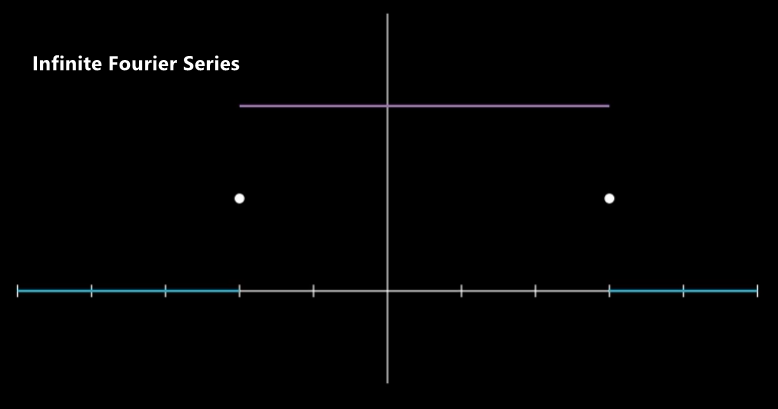
\includegraphics[height=5cm]{Fourier Infinite Fourier Series}
  \end{center}

  \topic{Orthogonality}\\
  Recall: The vectors
  \begin{align}
    u =
    \begin{bmatrix}
      u_1\\
      u_2\\
      \vdots\\
      u_n
    \end{bmatrix}
    \qquad \text{and} \qquad
    v =
    \begin{bmatrix}
      v_1\\
      v_2\\
      \vdots\\
      v_n
    \end{bmatrix}
  \end{align}

  are orthogonal if the dot product is zero.

  \begin{align}
    u \circ v & = \sum^n_{i = 1} u_i v_i = 0
  \end{align}

  We want to generalize this to function $x \in [-L, L]$.

  \dfn Two functions $f(x)$ and $g(x)$ are orthogonal on $[a, b]$ if

  \begin{align}
    \int^b_a f(x)g(x) \dx & = 0
  \end{align}

  \thm All basis functions in the Fourier Series are mutually orthogonal

  \begin{align}
    \int^L_{-L} \sin\Big(\frac{m \pi x}{L}\Big) \FS \dx & = 0 \quad n \neq m\\
    \int^L_{-L} \cos\Big(\frac{m \pi x}{L}\Big) \FC \dx & = 0 \quad n \neq m
  \end{align}
  What happens if $m = n$?
  \begin{align}
    \int^L_{-L} \sin^2\Big( \frac{m \pi x}{L} \Big) \dx
  \end{align}
  Here, we want to use the double angle formula: $\cos(2\theta) = 1 - 2\sin^2 \theta$.
  \begin{align}
    \int^L_{-L} \sin^2\Big( \frac{m \pi x}{L} \Big) \dx & =
    \frac{1}{2} \int^L_{-L} 1 - \cos\Big(\frac{2 m \pi x}{L}\Big) \dx\\ & =
    \frac{1}{2} \Big[ x - \frac{L}{2 m \pi}\sin\Big(\frac{2 m \pi x}{L}\Big)\Big]^L_{-L}\\ & =
    \frac{1}{2} \Big[L - \frac{L}{2 m \pi} \sin(2 m \pi) - \Big(-L - \frac{2}{2 m \pi} \sin(-2 m \pi)\Big)\Big]\\ & =
    L
  \end{align}
\end{document}
